\chapter{为什么说好的‘全球化’,现在却掀起了‘逆全球化’的浪潮?}

\section{引言:从“世界是平的”到“世界是碎的”}

在2005年,当《纽约时报》的专栏作家托马斯·弗里德曼(Thomas Friedman)出版他那本影响深远的著作《世界是平的》(The World Is Flat)时,全球化的浪潮正值巅峰。他描绘了一个激动人心的未来:柏林墙倒塌,互联网兴起,外包、离岸生产、全球供应链等十大“推土机”正在铲平各国之间的壁垒,创造一个公平竞争的平台。在这个平坦的世界里,无论你身在班加罗尔、北京还是波士顿,只要有才华和网络,就能参与全球竞争,共享繁荣。

这个愿景在当时看来无比真实。想象一下你手中的智能手机:它的操作系统可能由加州的谷歌或苹果公司设计,核心处理器来自台湾的台积电,内存芯片产自韩国的三星,摄像头模块或许是日本索尼的杰作,最后在中国深圳的工厂里由成千上万的工人组装完成,再通过覆盖全球的物流网络,销售到你所在的城市。这件小小的设备,就是全球化黄金时代的缩影——它集全球智慧与劳动力于一身,以普通人能够承受的价格,提供了前所未有的强大功能。这,就是全球化承诺的“福音”。

然而,仅仅十多年后,世界的图景似乎发生了惊人的逆转。2016年,英国公投“脱欧”(Brexit),高喊着“拿回控制权”(Take Back Control)的口号,选择离开这个全球最大的单一市场。同年,唐纳德·特朗普(Donald Trump)当选美国总统,他猛烈抨击全球贸易协定是“灾难”,称其“强暴”了美国经济,并对中国等国发动了声势浩大的贸易战。一时间,“美国优先”、“建墙”、“去风险化”(De-risking)等词语取代了“自由贸易”和“全球合作”,成为新的政治热词。世界似乎不再是平的,反而变得越来越“碎片化”。

这不禁让人陷入巨大的困惑:为什么曾经被精英阶层和主流媒体普遍赞誉,被视为通往繁荣与和平的康庄大道的全球化,现在却掀起了如此强烈的反对浪潮?那个承诺让所有人受益的“共赢”故事,为何在许多人听来,变成了一个关于“赢家”与“输家”的残酷叙事?

要解开这个谜团,我们不能仅仅停留在经济学的效率计算上,而必须深入全球化的政治维度,审视它如何像一场无声的革命,深刻地重塑了国家主权、国内的权力分配、社会结构乃至每个人的身份认同。正是这些被“效率”和“增长”光环所掩盖的政治影响,最终点燃了“逆全球化”的熊熊烈火。

\section{全球化:一场跨越时空的宏大叙事}

在我们深入剖析其政治后果之前,有必要清晰地认识到,我们今天所谈论的“全球化”并非新生事物,而是一个有着悠久历史的多维度进程。它并不仅仅是经济活动,更是一张交织着政治、文化和技术的复杂网络。

\subsection{历史上的全球化浪潮}

人类的连接从未停止。古代的丝绸之路,连接了东方与西方,交换的不仅是丝绸与香料,还有思想、宗教和技术。15世纪开始的“地理大发现”,则开启了第一波真正意义上的全球化浪潮,它由远洋航船驱动,将美洲的白银、非洲的劳动力和亚洲的商品卷入一个由欧洲主导的世界体系。

而我们今天所经历的,通常被称为“第三波全球化”或“超全球化”(Hyper-globalization),它始于20世纪80年代,并在冷战结束后达到顶峰。与前两次相比,这一波全球化有其鲜明的特征:

\begin{enumerate}
\item \textbf{技术革命的驱动:} 如果说上一波全球化由蒸汽机和电报驱动,那么这一波则由\textbf{集装箱、光纤电缆和互联网}驱动。
\begin{itemize}
\item \textbf{集装箱}的发明看似普通,却是一场物流革命。它将货物标准化的装进一个个铁盒子里,极大地降低了装卸成本和时间,使得远洋运输变得异常便宜。一件T恤从越南运到欧洲的成本,可能还不到一欧元。
\item \textbf{互联网和光纤电缆}则让信息的跨国流动成本降至几乎为零。这不仅意味着我们可以和地球另一端的朋友视频通话,更意味着一家纽约的公司可以将其客户服务或软件编程工作外包给印度的工程师,实时协同工作。
\end{itemize}
\item \textbf{政治意识形态的推动:} 冷战的结束,标志着市场经济和自由民主模式的“胜利”。以美国和英国为首的西方国家大力推行“新自由主义”(Neoliberalism)经济政策,其核心思想是:\textbf{放松管制、私有化、自由贸易}。这一思想通过世界贸易组织(WTO)、国际货币基金组织(IMF)和世界银行(World Bank)等国际机构,被推广到全球。各国纷纷降低关税、开放市场、欢迎外资,为商品和资本的自由流动扫清了政治障碍。
\end{enumerate}

\subsection{全球化的四个维度}

在技术和政治的双重驱动下,当代全球化呈现出四个紧密相连的维度:

\begin{itemize}
\item \textbf{经济全球化:} 这是最核心的维度。它不仅指商品贸易,更重要的是\textbf{全球生产链的形成}。一辆汽车可能包含来自30多个国家的零部件。资本的全球流动速度更是惊人,每天数万亿美元的资金在全球金融市场穿梭,寻找最高的投资回报。
\item \textbf{政治全球化:} 随着全球性问题(如气候变化、恐怖主义、金融危机、流行病)的增多,单一国家已无力应对。这催生了\textbf{全球治理}(Global Governance)的需求,国际组织(如联合国、WTO)、国际法庭和各类跨国非政府组织(NGO)的影响力日益增强。
\item \textbf{文化全球化:} 好莱坞电影、美剧、日本动漫、韩国K-Pop、星巴克咖啡和麦当劳快餐遍布全球,形成一种趋同的消费文化。但同时,它也激发了文化的“反向流动”,例如瑜伽在西方的流行,以及对本土文化保护的呼声。这种现象被称为“全球在地化”(Glocalization),即全球产品为了适应本地市场而做出改变。
\item \textbf{技术与社会全球化:} 社交媒体(Facebook, Twitter, TikTok)让普通人能够以前所未有的广度和速度进行跨国交流。跨国移民和旅游的普及,也让不同社会的人们有了更多面对面接触的机会。
\end{itemize}

在20世纪末的乐观氛围中,这四个维度的融合被认为将带来一个更美好、更富裕、更和平的世界。经济的相互依赖会减少战争的可能(“金拱门理论”),文化的交流会增进理解,技术的进步会赋能每一个人。然而,这个美好的愿景,却在现实的政治土壤中,结出了意想不到的苦果。

\section{ 全球化的政治代价:为何“逆流”涌动?}

全球化并非一场纯粹的经济活动,它本质上是一场深刻的政治变革。它重新定义了权力,改变了利益分配格局,并因此触动了现代国家最核心的根基。逆全球化浪潮的兴起,正是对这些政治代价的激烈反应。

\subsection{对国家主权的侵蚀:谁在替我们做决定?}

自1648年《威斯特伐利亚和约》签订以来,\textbf{国家主权}(National Sovereignty)——即国家在其领土内拥有至高无上的、排他性的权力——一直是国际关系的基石。然而,超全球化正在从三个方面系统性地侵蚀这一基石。

\textbf{第一,来自超国家机构的挑战。}

\begin{itemize}
\item \textbf{案例:欧盟与“布鲁塞尔的官僚”}
欧洲联盟(EU)是全球化最极致的实验。它创造了一个拥有4.5亿人口的庞大单一市场,实现了商品、服务、资本和人员的自由流动。但这种便利是有代价的:成员国需要将一部分主权“让渡”给位于布鲁塞尔的欧盟机构。欧盟的法律凌驾于成员国国内法之上,从农产品的标准、企业的环保要求到数据隐私保护(如GDPR),都由欧盟统一制定。
对于支持者来说,这是必要的“主权共享”,是为了获得更大的集体利益。但对于许多普通民众,尤其是英国的“脱欧派”而言,这意味着国家的命运被一群未经选举、远在天边的“布鲁塞尔官僚”所掌控。他们认为,英国无法自主决定自己的移民政策,无法自由地与其他国家签订贸易协定,甚至无法规定本国渔民在自己海域的捕鱼配额。因此,“拿回控制权”成为最有号召力的口号,它精准地击中了民众对主权流失的焦虑。

\item \textbf{案例:IMF的“结构性调整”}
对于发展中国家而言,主权受到的挑战则更为直接。在20世纪80、90年代,许多陷入债务危机的拉美和非洲国家,不得不向国际货币基金组织(IMF)求助。IMF的贷款并非无条件的,而是附带了一整套被称为“结构性调整计划”(SAPs)的严苛要求,包括:大规模私有化国有企业、削减教育和医疗等公共开支、取消对本国产业的保护、全面开放市场。
这些政策,被经济学家称为“华盛顿共识”,旨在将这些国家强行纳入全球市场体系。但从受援国的角度看,这无异于将国家的经济决策权拱手相让。这些由外国专家制定的政策,往往忽视了当地的具体国情,导致了大规模失业、社会动荡和贫富差距急剧扩大。在许多拉美民众的记忆中,IMF的干预是一段丧失经济主权、任人宰割的屈辱历史,这种集体记忆至今仍在影响着该地区的政治生态。
\end{itemize}

\textbf{第二,来自跨国公司的挑战。}

如果说超国家机构是对政治主权的挑战,那么跨国公司(TNCs)则是对经济主权的挑战。苹果、亚马逊、壳牌等巨型跨国公司的年收入,超过了世界上大多数国家的GDP。它们“用脚投票”的能力,赋予了它们对抗国家主权的巨大权力。
\begin{itemize}
\item \textbf{“监管套利”与“逐底竞争”:} 跨国公司可以在全球范围内配置资源,哪里税率最低,就把利润转移到哪里(如爱尔兰、开曼群岛);哪里环保法规最宽松,就把污染最严重的工厂设在哪里;哪里劳工权益最没有保障,就把生产线转移到哪里。这迫使各国政府为了吸引和留住投资,不得不展开一场“逐底竞争”(Race to the Bottom),竞相降低税收、放松管制。结果是,国家保护本国劳工和环境的能力被大大削弱。
\item \textbf{ISDS条款:公司的“法外治权”:} 许多双边或多边贸易协定中,都包含一项极具争议的条款——“投资者-国家争端解决机制”(ISDS)。该条款允许外国投资者,如果认为东道国的政策(如新的环保法规、提高最低工资)损害了其“可预期的利润”,就可以在超越该国司法体系的国际仲裁庭上起诉该国政府,并索取巨额赔偿。批评者认为,这相当于给了跨国公司一种“法外治权”,使其可以否决主权国家的公共政策,严重侵犯了民主决策的权力。
\end{itemize}

\textbf{第三,来自全球性问题的挑战。}
气候变化、网络攻击、全球疫情(如COVID-19)等问题,本质上是无视国界的。任何一个国家都无法单独解决。这看似需要更多的全球合作,但也反向凸显了国家主权的无力感。当本国政府无法有效保护民众免受这些外部威胁时,民众对政府的信任感就会下降,并可能转向更激进的、承诺“筑墙”来隔绝外部风险的政治力量。

\subsection{ 对国内就业的冲击:谁动了我的奶酪?}

如果说主权问题还略显抽象,那么全球化对就业和收入的冲击,则是每个普通人都能切身感受到的痛。经济学理论告诉我们,自由贸易能实现资源的最优配置,提升整体经济效率。但理论很少强调的是,\textbf{“整体”的收益,并不意味着“每个人”都能受益。}

\begin{itemize}
\item \textbf{案例:美国“铁锈地带”的衰落}
从宾夕法尼亚州、俄亥俄州到密歇根州,这片曾经是美国工业心脏的地带,如今被称为“铁锈地带”(Rust Belt)。在20世纪中叶,这里的钢铁厂、汽车厂和煤矿曾为数百万蓝领工人提供了稳定、体面、有工会保障的中产阶级生活。
然而,从20世纪80年代开始,全球化的浪潮袭来。日本和德国的汽车以其高效和低价,冲击着底特律的汽车巨头。更致命的是,随着贸易壁垒的降低,美国公司开始大规模地将生产线转移到劳动力成本更低的国家,先是墨西哥,2001年中国加入WTO后,更是以前所未有的规模流向中国。
结果是灾难性的。工厂成片倒闭,城市人口锐减,曾经繁华的社区变得萧条。那些为公司奉献了一生的工人,突然发现自己人到中年,身怀的屠龙之技(如炼钢、操作机床)在新经济中毫无用处。他们面临的选择,要么是长期失业,要么是去沃尔玛当一名薪水微薄的收银员。虽然整体经济(尤其是华尔街和硅谷)在增长,但他们的生活水平却在倒退,尊严也备受打击。

\item \textbf{“中国冲击”(China Shock)的实证研究}
这不仅仅是 anecdotal stories。麻省理工学院的经济学家戴维·奥特(David Autor)等人的著名研究“中国冲击”,通过严谨的数据分析,证实了这一点。他们发现,在1999年到2011年间,那些受中国进口商品冲击最严重的美国地区,其制造业就业岗位下降更剧烈,整体失业率更高,工人工资增长更慢。这项研究有力地说明,来自特定国家的贸易竞争,确实对特定地区的就业和社区造成了持久的、负面的影响。

\item \textbf{斯托尔帕-萨缪尔森定理的残酷现实}
这背后的经济学逻辑,可以用“斯托尔帕-萨缪尔森定理”(Stolper-Samuelson Theorem)来通俗地解释。该定理指出,当一个国家开放贸易时,该国\textbf{充裕}的生产要素(比如发达国家的资本和高技能劳动力)的价格会上升,而\textbf{稀缺}的生产要素(比如发达国家的低技能劳动力)的价格会下降。
翻译成大白话就是:在全球化中,发达国家的资本家、金融精英、软件工程师、科学家会因为全球市场而赚得盆满钵满;而那些从事简单重复劳动的蓝领工人,则不得不与来自发展中国家的、薪水要求低得多的工人竞争,其议价能力和工资水平自然会受到巨大压制。
\end{itemize}

这种结构性的失业和收入停滞,在“铁锈地带”等地区积累了长达数十年的怨气和绝望。当特朗普高喊“把工作带回美国”并承诺对进口商品征收高额关税时,他精准地回应了这些“被遗忘的人”的诉求。他们投票给特朗普,不仅是经济选择,更是一种政治反抗,是对那个忽视他们痛苦的全球化精英叙事的复仇。

\subsection{ 贫富差距的加剧:一个世界,两个极端}

全球化在创造巨大财富的同时,也以前所未有的方式加剧了财富分配的不平等,无论是在发达国家内部,还是在发展中国家内部。

\begin{itemize}
\item \textbf{“大象曲线”揭示的全球赢家与输家}
世界银行前首席经济学家布兰科·米兰诺维奇(Branko Milanović)提出的“大象曲线”(Elephant Chart)直观地揭示了这一现象。该图表展示了1988年至2008年这二十年全球化黄金时期,全球不同收入阶层的人口,其实际收入增长情况。


\begin{figure}[h!]
    \centering
    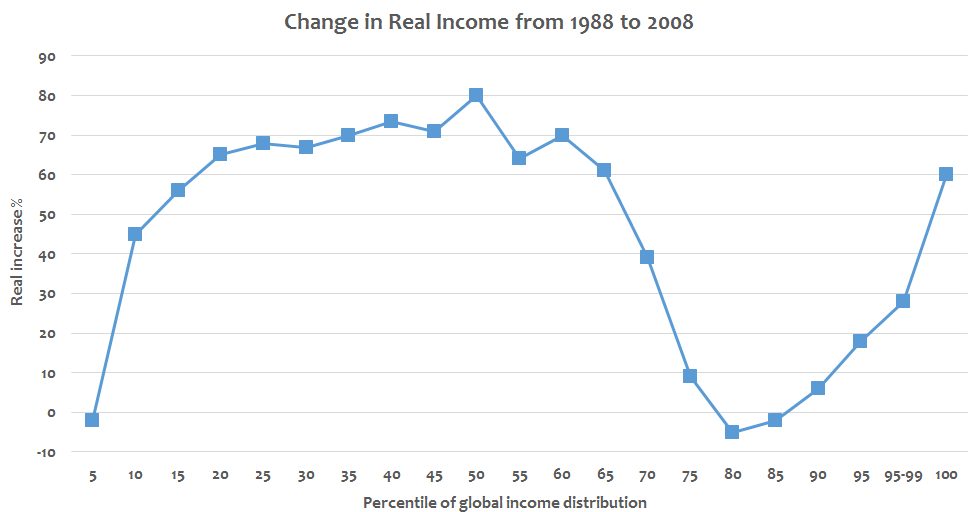
\includegraphics[width=\textwidth]{elephant_chart.png}
    \caption{Elephant Chart}
    \label{fig:elephant_chart}
\end{figure}

这条曲线看起来像一头大象:
\begin{itemize}
\item \textbf{象鼻高高翘起:} 全球收入最高的1\%(全球精英),他们的收入增长了超过60\%。他们是全球化的最大赢家。
\item \textbf{象背高高隆起:} 位于全球收入中段的人群,主要是以中国为代表的新兴经济体的中产阶级,他们的收入实现了惊人的增长,很多人实现了翻番甚至更多。这是全球化最值得称道的成就——数亿人脱离了贫困。
\item \textbf{象鼻与象背之间的低谷:} 位于全球收入分配高端(大约75-90百分位)的人群,他们的收入增长几乎为零,甚至为负。这部分人,恰恰就是\textbf{发达国家的下层和中产阶级}。
\end{itemize}

“大象曲线”清晰地告诉我们:全球化的果实,被全球最富有的那一小撮人和发展中国家的新兴中产阶级所分享,而发达国家的普通劳动者,则成了被遗忘的“输家”。

\item \textbf{发达国家内部的两极分化}
在美国等发达国家,CEO的薪酬与普通员工的薪酬差距,从几十倍拉大到几百倍。资本的回报率(利息、股息、资本利得)持续高于劳动回报率(工资),这是法国经济学家托马斯·皮凯蒂(Thomas Piketty)在《21世纪资本论》中揭示的核心趋势。全球化加剧了这一趋势:资本可以全球流动避税,而劳动力则基本被困在原地。工会力量因企业可以轻易将工厂外迁的威胁而被削弱,政府也不敢对资本和富人征收重税,担心他们会“逃离”。

\item \textbf{发展中国家内部的撕裂}
即使是在作为“赢家”的发展中国家,全球化也带来了内部的巨大撕裂。少数与全球市场接轨的精英、出口导向型企业主和生活在沿海大城市的人群迅速暴富,而广大的内陆地区、农村人口和传统产业的从业者,则可能被边缘化。中国的城乡差距、印度的阶级固化,都在全球化时代被进一步拉大。
\end{itemize}

当一个社会大部分的经济增长果实只被少数人攫取,当社会流动性下降,普通人无论如何努力都无法改善生活时,社会的公平感和正义感就会被侵蚀,对现有政治经济体制的愤怒和不信任感就会滋生,为民粹主义和激进政治的兴起提供了最肥沃的土壤。

\subsection{文化认同的冲击:我是谁?我们是谁?}

全球化不仅是商品和资本的流动,也是文化、价值观和生活方式的流动。这种流动在促进交流的同时,也引发了深刻的文化焦虑和认同危机。

\begin{itemize}
\item \textbf{“文化帝国主义”的担忧}
以好莱坞、麦当劳、星巴克为代表的西方消费文化,随着全球化席卷全球。这在一些国家引发了对“文化帝国主义”的担忧,认为本土的文化传统、语言和价值观正在被同质化的、强势的西方文化所侵蚀。
\begin{itemize}
\item \textbf{案例:法国的“文化例外”}
法国长期以来都奉行“文化例外”(l'exception culturelle)政策,坚称文化产品不是普通商品,不能完全遵循自由贸易原则。为了抵御好莱坞的冲击,法国政府通过补贴、税收优惠和规定电台必须播放一定比例的法语歌曲、影院必须排映一定比例的法国电影等方式,来保护和扶持本国的文化产业。这正是对文化全球化的一种自觉抵制。
\end{itemize}

\item \textbf{移民带来的社会张力}
全球化带来的人员流动,尤其是大规模的移民,深刻地改变了许多西方社会的人口结构。虽然移民为社会带来了劳动力和多样性,但也引发了关于资源分配、社会融合和国家认同的激烈争论。
\begin{itemize}
\item \textbf{案例:欧洲的移民危机与右翼崛起}
2015年,大量来自中东和北非的难民涌入欧洲,引发了严重的社会和政治危机。在许多欧洲民众看来,大规模的、文化背景迥异的移民,不仅对本国的福利体系、社会治安构成了压力,更重要的是,它挑战了“我们是谁”这个根本问题。德国的“我们能做到”(Wir schaffen das)的开放政策,与匈牙利等国修建边境墙的强硬做法,形成了鲜明对比。
欧洲各国的右翼民粹政党,如法国的国民联盟、德国的选择党,正是利用了民众的这种不安和恐惧。他们将移民问题与恐怖主义、失业和文化丧失等问题捆绑在一起,将自己塑造为“本土文化”和“国家认同”的捍卫者,从而获得了大量选票。
\end{itemize}

\item \textbf{“全球化主义者” vs. “本土主义者”}
英国学者戴维·古德哈特(David Goodhart)提出了一个极具解释力的概念框架,他将社会分为了两类人:“无根的全球化主义者”(Anywheres)和“有根的本土主义者”(Somewheres)。
\begin{itemize}
\item \textbf{Anywheres(世界公民):} 他们通常受过高等教育,从事专业性工作,流动性强,视野全球化。他们从全球化中受益,认同开放、多元、包容的普世价值。他们感觉自己既可以属于伦敦,也可以属于纽约或上海。
\item \textbf{Somewheres(本土居民):} 他们是社会的大多数,受教育程度相对较低,生活和工作与特定的“地方”(家乡、社区)紧密相连。他们的身份认同根植于本土的传统、文化和社群关系。他们感觉被全球化浪潮所抛弃和威胁,他们的价值观(如家庭、宗教、国家)被“Anywheres”所鄙视。
\end{itemize}
\end{itemize}

脱欧公投和特朗普的当选,在很大程度上可以被看作是人数众多的“Somewheres”对人数较少但掌控话语权的“Anywheres”的一场政治反叛。这解释了为什么许多投票支持脱欧或特朗普的地区,恰恰是那些经济上受全球化冲击最严重、同时在文化上感觉被忽视的地区。

\section{全球化的赢家与输家:一幅残酷的众生相}

综合以上分析,我们可以清晰地勾勒出全球化这场盛宴中的“赢家”与“输家”。它从来不是一场普惠所有人的派对,而是一场深刻的利益重分配。

\begin{itemize}
\item \textbf{主要赢家:}
\begin{itemize}
\item \textbf{跨国公司及其高管/股东:} 他们是全球化的总设计师和最大受益者。通过全球布局,他们实现了成本最小化和利润最大化。
\item \textbf{全球金融精英:} 华尔街的银行家、基金经理们,通过资本的全球自由流动,创造和积累了惊人的财富。
\item \textbf{发达国家的高技能专业人士:} 硅谷的工程师、律师、顾问等“知识工人”,他们的技能在全球市场中具有稀缺性,因而获得了高额回报。
\item \textbf{成功融入全球产业链的发展中国家(及其部分国民):} 以中国、越南等为代表的国家,通过承接制造业转移,实现了经济的飞速增长,创造了庞大的新兴中产阶级,数亿人摆脱了绝对贫困。这是全球化最积极、最不可否认的成就。
\item \textbf{全球消费者(在一定程度上):} 享受到了来自世界各地的、前所未有地廉价和多样化的商品。
\end{itemize}

\item \textbf{主要输家:}
\begin{itemize}
\item \textbf{发达国家的蓝领工人和低技能劳动者:} 他们是全球化最直接的受害者,面临失业、工资停滞和职业尊严的丧失。
\item \textbf{未能融入全球经济的发展中国家(及其大部分国民):} 许多非洲和拉美的国家,在全球化中被进一步边缘化。它们没有强大的制造业基础,只能出口初级原材料,在全球分工中处于最底层,国内贫困问题依然严峻。
\item \textbf{受冲击的本土中小企业:} 它们无力与拥有巨大规模和成本优势的跨国公司竞争,在本国市场也面临被挤压的困境。
\item \textbf{地球环境:} 全球生产和消费的极大扩张,以及廉价的跨国运输,加剧了碳排放、资源消耗和环境污染。污染密集型产业从监管严格的发达国家转移到监管宽松的发展中国家,形成了“污染天堂”。
\end{itemize}
\end{itemize}

当“输家”群体的数量和怨气积累到一定程度,并且他们的声音能够通过民粹主义政治家被有效动员起来时,“逆全球化”的浪潮便不可避免地到来了。

\section{逆全球化浪潮:表现、动因与未来}

当前的“逆全球化”浪潮,并非要让世界退回到各国老死不相往来的孤立状态,这在技术上和经济上都已不可能。它更像是一次对过去三十年“超全球化”模式的激烈修正和重塑。

\begin{itemize}
\item \textbf{主要表现:}
\begin{itemize}
\item \textbf{贸易保护主义抬头:} 最典型的就是特朗普政府发动的对华贸易战,大规模加征关税。但这种做法并非美国独有,印度、巴西等国也在提高关税,欧盟则通过“碳边境调节机制”(CBAM,即碳关税)等新型贸易壁垒来保护自身产业。
\item \textbf{供应链的“去风险化”与“区域化”:} COVID-19疫情暴露了全球供应链的脆弱性——当某个环节(如中国的港口)中断,全球生产都可能陷入停滞。俄乌冲突则让各国意识到将供应链过度集中于“地缘政治对手”的风险。因此,各国政府和企业开始推动供应链的调整,从过去单纯追求“效率”转向追求“安全”和“韧性”。
\begin{itemize}
\item \textbf{近岸外包(Near-shoring):} 将生产线从遥远的亚洲迁回离本国更近的地区(如美国公司迁往墨西哥)。
\item \textbf{友岸外包(Friend-shoring):} 将供应链集中在政治上可信赖的盟友国家。
\item \textbf{产业政策回归:} 各国政府不再羞于谈论“产业政策”,而是通过巨额补贴来扶持本国的关键产业,如美国的《芯片与科学法案》和《通胀削减法案》,旨在将半导体和新能源产业吸引回本土。
\end{itemize}
\item \textbf{民族主义和民粹主义政治的常态化:} “本国优先”的口号在全球范围内流行。政治家们通过煽动排外情绪、强调国家利益至上,来获取国内政治支持。
\item \textbf{全球合作的困境:} 在气候变化、公共卫生、核不扩散等亟需全球合作的领域,大国间的战略竞争和不信任感,使得达成和执行有意义的国际协议变得异常困难。
\end{itemize}

\item \textbf{未来展望:一个“有管理的全球化”?}
未来的全球化,可能不再是过去那种野蛮生长的、无限制的自由流动。它可能会呈现出以下几个特征:
\begin{enumerate}
\item \textbf{更具选择性:} 国家会在数字、金融等领域保持开放,但在涉及国家安全和关键技术的领域,则会加强保护和管制。
\item \textbf{更加区域化:} 以欧盟、北美(USMCA)、东亚(RCEP)为核心的三大区域经济集团的内部联系会更加紧密,而跨区域的联系则可能面临更多障碍。
\item \textbf{更加注重公平与安全:} 国内的公平分配问题(如何补偿全球化中的输家)和供应链的安全问题,将被置于比单纯追求经济效率更优先的位置。
\item \textbf{更加政治化:} 经济决策将越来越多地服务于地缘政治目标,国家安全考量将深刻影响贸易和投资的流向。
\end{enumerate}
\end{itemize}

\section{结论:在断裂的世界中重新思考连接}

全球化,这把曾经被认为是能斩断贫困与冲突的“利剑”,终究显露了它的“双刃”本质。它在连接世界、创造财富的同时,也切断了许多人与稳定工作、与家乡社区、与传统认同之间的纽带。它带来的巨大经济收益,与它造成的深刻政治创伤,共同构成了我们这个时代的复杂面貌。

“逆全球化”的浪潮,正是这些被全球化叙事所忽视、所压抑的政治创伤的总爆发。它是对主权流失的焦虑、对经济不公的愤怒、对文化失落的恐慌的集体回应。它提醒我们,任何经济模式如果不能在政治上和社会上获得持续的合法性,终将是不可持续的。

理解了全球化如何通过冲击经济和主权来催生政治反抗,我们便能更好地把握当今世界政治的核心矛盾。然而,故事还未结束。当这些由全球化带来的经济和文化上的不安全感,与一个社会内部早已存在的、更深层次的身份裂痕——如种族、宗教、地域——相互交织时,又会引爆怎样更具破坏性的政治能量?为什么在许多国家,政治辩论的核心已经从“我们应该做什么”(政策),变成了“我们是谁”(身份)?为什么“你来自哪里”似乎比“你是谁”更加重要?

这,正是我们下一章将要深入探讨的,当代政治的另一个幽灵——“身份政治”。